%%%%%%%%%%%%%%%%%%%%%%%%%%%%%%%%%%%%%%%%%%%%%%
%
% Modelo LaTeX criado por Bruno Ferreira
%
%%%%%%%%%%%%%%%%%%%%%%%%%%%%%%%%%%%%%%%%%%%%%%

\documentclass[11pt, a4paper, twoside]{article}

%%%%%%%%%%%%%%%%%%%%%%%%%%%%%%%%%%%%%%%%%%%%%%
%% definição das packages a usar

% definir novo package:
% \usepackage[options]{args}

% hifenização e outras especificações para português
\usepackage[portuguese]{babel}

% hiperligações
\usepackage{hyperref}
\hypersetup{colorlinks=true, urlcolor=blue, linkcolor=black}

% escrever acentos e coisas do género sem que o latex se desoriente
\usepackage[utf8]{inputenc}

% para ter imagens, depois define a directoria de imagens
\usepackage{graphicx}
\graphicspath{{./imagens/}}

\usepackage[labelformat=empty]{caption}
\usepackage[labelformat=empty]{subcaption}

% para ter a informação de quantas páginas tem o documento
\usepackage{lastpage}

% definir o cabeçalho e rodapé
\usepackage{fancyhdr}
\pagestyle{fancy}
\fancyhead[L]{\small{Haskassonne}}
\fancyhead[R]{\small{Laboratórios de Informática I}}

% ter enumerações alinhadas
\usepackage{enumitem}

% escrever algoritmos
\usepackage[algoruled]{algorithm2e}

% definir comandos especiais
\newcommand\doubleplus{+\kern-1.3ex+\kern0.8ex} %


%%%%%%%%%%%%%%%%%%%%%%%%%%%%%%%%%%%%%%%%%%%%%%
%% inicio do documento
\begin{document}
\title{Haskassonne}
\date{\today}
\author{
  Bruno Alexandre Alves Ferreira\\
  \texttt{a61055@alunos.uminho.pt}
  \and
  Nuno Miguel Oliveira Salvador\\
  \texttt{a48398@alunos.uminho.pt}
  \and
  Grupo 007
}

\maketitle
\begin{abstract}
\begin{center}
  Esta é uma implementação em Haskell do Carcassone.
\end{center}
\end{abstract}
\newpage

\tableofcontents

\newpage
\section{Resumo}

Neste relatório encontram-se explicitadas de forma detalhada as escolhas do \textit{grupo 007} no que ao projecto da unidade curricular de Laboratórios de Informática I diz respeito. Serão revistas as escolhas em relação aos tipos de dados usados, a forma como se interligam nos vários programas e outras decisões tomadas para resolver o problema que nos foi proposto.

\newpage
\section{Introdução}

Pretende-se implementar, em Haskell, uma versão simplificada do famoso jogo de tabuleiro Carcassonne. Esta versão simplificada contém apenas 4 tipos distintos de peças e não contempla estradas.

\begin{figure}[h!]
\centering
\begin{subfigure}{.25\textwidth}
  \centering
  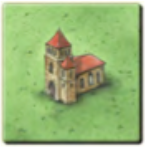
\includegraphics[width=0.8\linewidth]{tileB}
  \caption{Peça B}
\end{subfigure}%
\begin{subfigure}{.25\textwidth}
  \centering
  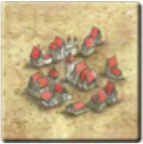
\includegraphics[width=0.8\linewidth]{tileC}
  \caption{Peça C}
\end{subfigure}%
\begin{subfigure}{.25\textwidth}
  \centering
  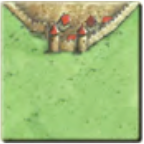
\includegraphics[width=0.8\linewidth]{tileE}
  \caption{Peça E}
\end{subfigure}%
\begin{subfigure}{.25\textwidth}
  \centering
  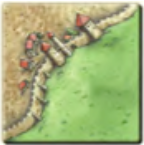
\includegraphics[width=0.8\linewidth]{tileN}
  \caption{Peça N}
\end{subfigure}%
\end{figure}

De forma resumida, o Carcassonne é um jogo de tabuleiro que se expande à medida que o jogo avança. O jogo começa com uma única peça em jogo. No seu turno, os jogadores devem retirar aleatoriamente uma nova peça e coloca-la adjacente a uma peça do terreno. Esta nova peça deve ser colocada de forma concordante com as peças que lhe são adjacentes.

Depois de colocar a sua peça em jogo, o jogador pode optar por colocar um \textit{meeple} numa parte da peça colocada e assim dominar aquela zona. O jogador não pode colocar um \textit{meeple} numa zona dominada por outro \textit{meeple}, no entanto pode acontecer que zonas dominadas por jogadores diferentes passem a ser partilhadas quando se coloca uma nova peça que junte duas zonas.

O jogo termina quando a ultima peça é colocada, ou quando não é possível colocar as restantes peças. Nesse momento, todas as zonas são pontuadas para o jogador que as domina. O jogador com mais pontos ganha o jogo.

\newpage
\section{Desenvolvimento do Projecto}

\subsection{Requisitos}

Para implementar o Haskassonne, este foi dividido em 3 fases mais simples.
Todas estas fases recebem como input um ficheiro XML representante do estado actual do jogo.

\begin{description}[style=multiline,leftmargin=1.5cm,font=\bfseries]
    \item[Draw] Imprimir uma representação do terreno em texto simples.
    \item[Play] Produzir uma jogada válida para o jogador actual.
    \item[Next] Escolher o tipo da próxima peça a ser jogada ou, caso o jogo tenha terminado, calcular as pontuações dos jogadores e remover todos os \textit{meeples}.
\end{description}

Torna-se assim possível executar os programas \textit{Play} e \textit{Next} repetidamente para conseguir sucessivas jogadas. Pode-se a qualquer momento fornecer o estado ao \textit{Draw} e obter uma representação visual das peças colocadas e dos \textit{meeples} em campo.

\subsection{Principais Tipos de Dados}

Ao longo do relatório faremos várias referências aos tipos de dados usados ou aos elementos que eles representam, assim sendo considerou-se essencial a sua explicação numa fase inicial do relatório.

Estes tipos de dados são usados para conseguir uma representação simplificada, em Haskell, da representação fornecida em XML. Existe, no nosso projecto, um módulo responsável por converter um ficheiro XML na representação interna e um segundo módulo que realiza a funcionalidade inversa.

\subsubsection[Player]{Player (módulo Leitor)}

Representa um jogador, que é identificado por um número inteiro entre zero e nove, inclusive. O jogador tem também uma pontuação.

\begin{description}[style=multiline,leftmargin=3cm,font=\bfseries]
    \item[s\_player::Int] Identificação do jogador.
    \item[s\_score::Int] Pontuação do jogador.
\end{description}

\subsubsection[Next]{Next (módulo Leitor)}

Informações obtidas na tag \textit{next} do XML do estado.

\begin{description}[style=multiline,leftmargin=2.5cm,font=\bfseries]
    \item[n\_tile::Char] A peça que deve ser colocada na próxima jogada.
\end{description}

\subsubsection[Meeple]{\textit{Meeple} (módulo Leitor)}

Um \textit{meeple} é um marcador que um jogador pode optar por colocar numa zona de um \textit{tile} que acabou de jogar. Este \textit{meeple} é que permite aos jogadores pontuar.

Um \textit{meeple}, com informação sobre o seu dono e tipo. O tipo do \textit{meeple} (Farmer, Knight ou Monk) define a zona onde este está colocado num \textit{Tile}.

\begin{description}[style=multiline,leftmargin=3cm,font=\bfseries]
    \item[m\_player::Int] Identificação do jogador.
    \item[m\_type::Char] O tipo do \textit{meeple} (F, K ou M).
\end{description}

\subsubsection[Tile]{\textit{Tile} (módulo Leitor)}

Um \textit{tile} representa uma peça do terreno.

\begin{description}[style=multiline,leftmargin=5.5cm,font=\bfseries]
    \item[t\_type::Char] O tipo da peça (B, C, E ou N).
    \item[t\_x::Int] A posição horizontal da peça.
    \item[t\_y::Int] A posição vertical da peça.
    \item[t\_orientation::] A orientação da peça (N, S, W ou E).
    \item[t\_meeple::Maybe Meeple] Um \textit{meeple}, caso exista.
\end{description}

\subsubsection[Board]{\textit{Board} (módulo Leitor)}

Representa um estado do tabuleiro, com os \textit{tiles}, \textit{meeples}, jogadores e informações sobre a próxima jogada.

\begin{description}[style=multiline,leftmargin=3.5cm,font=\bfseries]
    \item[b\_terrain::[Tile{]}] As peças em jogo.
    \item[b\_scores::[Player{]}] Os jogadores.
    \item[b\_next::Next] Informações sobre a próxima jogada.
\end{description}

\subsubsection[Map]{\textit{Map} (módulo Leitor)}

Uma matriz de \textit{Maybe Tile} para representar um mapa. Nesta representação as peças estão organizadas de acordo com os seus campos \textit{t\_x} e \textit{t\_y}.

Existe a possibilidade de não existir um \textit{tile} numa posição (x,y), daí a necessidade de ter a matriz de \textit{Maybe Tile}.

\begin{description}[style=multiline,leftmargin=3.5cm,font=\bfseries]
    \item[[[Maybe Tile{]]}] Matriz com os \textit{tiles} em jogo.
\end{description}

\newpage
\subsection{Tipos de Dados Auxiliares}

Estes tipos de dados têm um papel menos significativo. No entanto facilitam a execução de alguma tarefas.

\subsubsection[Limits]{Limits (módulo Leitor)}

Representa os limites exteriores do mapa.

\begin{description}[style=multiline,leftmargin=3cm,font=\bfseries]
    \item[l\_Xmin::Int] Valor mínimo para o X.
    \item[l\_Xmax::Int] Valor máximo para o X.
    \item[l\_Ymin::Int] Valor mínimo para o Y.
    \item[l\_Ymax::Int] Valor máximo para o Y.
\end{description}

\subsubsection[Location]{Location (módulo Leitor)}

\begin{description}[style=multiline,leftmargin=2cm,font=\bfseries]
    \item[(Int, Int)] Localização (x,y) de um \textit{tile}.
\end{description}

\subsubsection[ScoredTile]{ScoredTile (módulo Pontuar)}

Um par constituído por (Zone, Int). Com este par torna-se mais fácil relacionar uma zona com o número de pontos que lhe está associado.

\begin{description}[style=multiline,leftmargin=2cm,font=\bfseries]
    \item[::Zone] Representa uma zona.
    \item[::Int] A pontuação atribuída a essa zona.
\end{description}

\subsubsection[Zone]{Zone (módulo Tabuleiro)}

Representa uma zona do mapa: uma cidade, um campo ou um claustro.

O primeiro \textit{tile} identifica a peça por onde se começou a zona. Os \textit{tiles} seguintes identificam os \textit{tiles} por onde se estende a mesma zona (neste conjunto deve estar incluído o \textit{tile} onde a zona começou).

No caso do claustro considera-se a zona como os 8 \textit{tiles} à volta do claustro e o próprio claustro.

Definem-se da seguinte forma:
\begin{description}[style=multiline,leftmargin=5cm,font=\bfseries]
    \item[City Tile [Tile{]}] Representa uma cidade.
    \item[Field Tile [Tile{]}] Representa um campo.
    \item[Cloister Tile [Tile{]}] Representa um claustro.
\end{description}

\subsubsection[Side]{Side (módulo Tabuleiro)}
Representa uma lateral de uma peça.

Isto facilita o reconhecimento de todos os \textit{tiles} de uma zona.

Define-se da seguinte forma:
\begin{description}[style=multiline,leftmargin=3cm,font=\bfseries]
    \item[SideField] Representa uma lateral de campo.
    \item[SideCity] Representa um campo.
    \item[SideBoth] Representa um claustro.
\end{description}

\subsubsection[Sides]{Sides (módulo Tabuleiro)}

Representa as laterais de uma peça.

\begin{description}[style=multiline,leftmargin=5cm,font=\bfseries]
    \item[(Side, Side, Side, Side)] Representa as laterais de um \textit{tile}.
\end{description}

\subsubsection[Art]{Art (módulo ArtASCII)}

\begin{description}[style=multiline,leftmargin=2cm,font=\bfseries]
    \item[[String{]}] Representa um tile em formato de texto simples.
\end{description}

\newpage
\subsection{Módulos}

\subsubsection{Leitor}
Utiliza o módulo \emph{Text.XML.Light} para converter os dados XML para os tipos de dados adaptados ao problema.

\subsubsection{Tabuleiro}
Contém uma série de utilitários para manipulação do tabuleiro.

\subsubsection{ArtASCII}
Permite o desenho do terreno em formato de texto simples.

\subsubsection{Escritor}
Tem a funcionalidade inversa ao módulo \emph{Leitor}: converter os dados (organizados em tipos de dados adaptados ao problema) para um tipo de dados intermédio que depois o módulo \emph{Text.XML.Light} consegue converter para XML.

\subsubsection{Pontuar}
Contém utilitários para contagem e atribuição de pontuação.

\subsubsection{FakePrettyShow}
Define uma função \emph{ppShow} que faz apenas um \emph{show}. Este módulo é importado em vez do \emph{Text.Show.Pretty} quando se quer submeter programas no Mooshak (o Mooshak não suporta \emph{Text.Show.Pretty}).

\newpage
\subsection{Programa Draw}
Descreve-se agora o funcionamento geral do programa Draw.\\

\begin{algorithm}[H]
  \SetKwInOut{Input}{input}
  \SetKwFunction{ConvertMaybeTileToArt}{convertMaybeTileToArt}
  
  \Input{XML com o estado atual}
  
  \BlankLine
  importa o XML para um Board\\
  obtém os limites exteriores do Board\\
  constroi o Map
  \BlankLine
  Matriz de Art$\leftarrow$\ForAll{maybeTiles of Map}{
    \ConvertMaybeTileToArt
  }
  imprime a Matriz de Art
  \caption{Funcionamento geral do Draw}
\end{algorithm}

\newpage
\subsection{Programa Play}
Descreve-se agora o funcionamento geral do programa Play.\\

\begin{algorithm}[H]
  \SetKwInOut{Input}{input}
  \SetKwData{Escolhido}{tileEscolhido}
  \SetKwData{Possiveis}{tilesPossiveis}
  \SetKwData{TipoCerto}{tipoDefinido}
  \SetKwFunction{TileAleatorio}{tileAleatorioDoTipo}
  
  \Input{XML com o estado atual}
  \BlankLine
  importa o XML para um Board\\
  \TipoCerto$\leftarrow$tipo da próxima peça a ser jogada.\\

  \BlankLine
  \eIf{não existem peças em jogo}{
    \Escolhido$\leftarrow$\TileAleatorio{'E'} na posição (0,0)
  }(\tcc*[f]{existem peças em jogo}){
    \Possiveis$\leftarrow$todos os tiles que podem ser jogados\\
    \If{jogador pode colocar Meeple}{
        \Possiveis$\leftarrow$\Possiveis \doubleplus tiles possíveis com meeples
    }
    \Escolhido$\leftarrow$seleccionar aleatoriamente um dos \Possiveis
  }
  
  \BlankLine
  \eIf{não recebeu nenhum argumento}{
    converte o \Escolhido para uma tag XML e imprime-a
  }{
    adiciona o \Escolhido ao Board\\
    converte o Board num Element\\
    imprime o Element em formato XML
  }
  \caption{Funcionamento geral do Play}
\end{algorithm}
\ \\
\ \\
A nossa implementação do programa Play tem uma funcionalidade extra: quando lhe é passado qualquer argumento, imprime um ficheiro de estado XML completo, em vez de apenas a tag com o \emph{Tile} jogado. Esta alteração permite-nos encaminhar o output do programa Play para o programa Next e assim jogar uma "ronda".


\newpage
\subsection{Programa Next}
Descreve-se agora o funcionamento geral do programa Next.\\

\begin{algorithm}[H]
  \SetKwInOut{Input}{input}
  \SetKwData{Escolhido}{tile}
  \SetKwData{Possiveis}{tilesPossiveis}
  \SetKwData{TipoCerto}{tipoEscolhido}
  \SetKwFunction{TileAleatorio}{tileAleatorioDoTipo}
  
  \Input{XML com o estado atual}
  \BlankLine
  importa o XML para um Board\\
  \TipoCerto$\leftarrow$tipo da próxima peça a ser jogada.\\

  \BlankLine
  \eIf{podem ser jogadas mais peças}{
    \Possiveis$\leftarrow$todos os tiles que podem ser jogados\\
    \Escolhido$\leftarrow$seleccionar aleatoriamente um dos \Possiveis\\
    \TipoCerto$\leftarrow$tipo do \Escolhido\\
    alterar o Next do Board com o \TipoCerto\\
    pontuar as cidades completas\\
    pontuar os claustros completos\\
    converte o Board num Element\\
  }(\tcc*[f]{jogo terminou}){
    colocar no Next do Board o tipo '-'\\
    pontuar as cidades\\
    pontuar os claustros\\
    pontuar os campos\\
    converte o Board num Element\\
  }
  
  \BlankLine
  \eIf{não recebeu nenhum argumento}{
    imprime o Element em formato XML (numa linha)
  }{
    imprime o Element em formato XML (legível)
  }
  \caption{Funcionamento geral do Next}
\end{algorithm}
\ \\
\ \\
A nossa implementação do programa Next tem uma funcionalidade extra: quando lhe é passado qualquer argumento, imprime um ficheiro de estado XML legível (com várias linhas e tabulações), em vez de um XML \emph{"one-liner"}. Esta alteração permite-nos ler e interpretar manualmente o ficheiro XML de forma mais rápida.

Colocar um '-' no \emph{Next} do \emph{Board} faz com que o módulo \emph{Escrever} o ignore, resultando num formato XML sem a tag next.

\newpage
\subsection[Zones]{\emph{Zones}}
Quando precisamos de calcular uma \emph{Zone} (cidade ou campo) fazemos uma pesquisa breadth-first que começa no \emph{Tile} que tem o \emph{meeple} e percorre todos os \emph{tiles} adjacentes que tenham laterais concordantes.

A \emph{Zone} de um claustro são os 8 tiles adjacentes ao claustro e o próprio claustro.

Este tipo de dados e forma de resolver o problema permitem-nos depois dar diversos usos à \emph{Zone}:

\begin{itemize}
  \item Contar o número de \emph{tiles} numa zona consiste em contar o número de elementos na lista de \emph{tiles}. No caso do claustro, deve-se subtrair um ao número de elementos nessa lista.
  \item Todas as zonas com os mesmos elementos na lista de \emph{tiles} são dominadas por mais que um meeple. Isto permite-nos saber quantos \emph{meeples} de cada jogador dominam uma zona e atribuir correctamente os pontos.
  \item Remover o \emph{meeple} que domina uma zona consiste em obter a localização do tile inicial da \emph{Zone}, pesquisar o \emph{tile} com essa localização no Board, remover o \emph{meeple} e adicionar uma unidade ao número de \emph{meeples} disponíveis desse jogador.
\end{itemize}

O algoritmo que verifica se uma cidade já está completa (no programa Next) é bastante semelhante, utilizando uma pesquisa breadth-first que percorre apenas os \emph{tiles} de cidade e termina caso a cidade não esteja completa ou quando não houver mais \emph{tiles} na orla (que significa que a cidade está completa).

\newpage
\section{Makefile}
A \emph{Makefile} contém várias regras principais:

\begin{description}[style=multiline,leftmargin=2cm,font=\bfseries]
    \item[all] Compila os três programas.
    \item[clean] Apaga ficheiros binários e temporários.
    \item[draw] Compila o programa Draw.
    \item[play] Compila o programa Play.
    \item[next] Compila o programa Next.
    \item[doc] Gera a documentação para as classes do projecto.
\end{description}

\newpage
\section{Testes}

\subsection{Ficheiro TestDraw.hs}
Foi feita uma tentativa de utilizar o QuickCheck no nosso projecto. Não nos ocorreram formas intuitivas de testar funcionamento complicado usando a geração de dados aleatórios, por isso os nossos testes usando QuickCheck resumem-se a testar se a rotação de Art e a remoção de duplicados em listas funciona.

Por outro lado a nossa script de jogar uma ronda providenciou-nos todo o tipo de situações para testar o nosso projecto.

\subsection{Ficheiros XML de teste}
Foram criados vários ficheiros XML para testes na directoria test. Estes servem para testar algumas funcionalidades básicas do programa, sendo que as mais avançadas foram testadas usando a script de jogar uma ronda.

\subsection{Script: Jogar uma ronda}
Foi criada uma script que "joga uma ronda". Caso não exista nenhum XML de estado, esta script começa por usar o ficheiro de testes com um tabuleiro vazio.

A script executa em sequência os programas Play e Next, executando antes e depois o programa Draw. Utilizando as funcionalidades extra que foram adicionadas aos programas Play e Next (que são activadas quando se fornece um argumento a estes programas) e gravando os vários XML que são produzidos pelos programas, conseguimos ter todo o tipo de testes e situações para por a nossa solução à prova.

Antes de terminar, a script coloca lado a lado o output do programa Draw antes e depois de jogar a ronda. Assim consegue-se ter uma perspectiva geral rápida sobre a evolução do jogo.

O verdadeiro potencial desta script é realizado quando ela é executada várias vezes. Desta forma consegue-se, partindo de um tabuleiro vazio chegar a um tabuleiro de fim de jogo, jogando ronda após ronda.

\newpage
\section{Elementos do Grupo}

\begin{figure}[h!]
\centering
\begin{subfigure}{.5\textwidth}
  \centering
  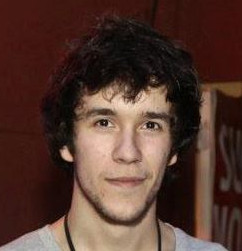
\includegraphics[width=0.8\linewidth]{brunoferreira}
  \caption{Bruno Ferreira (a61055)}
\end{subfigure}%
\begin{subfigure}{.5\textwidth}
  \centering
  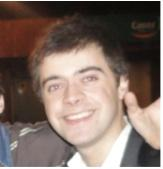
\includegraphics[width=0.8\linewidth]{nunosalvador}
  \caption{Nuno Salvador (a48398)}
\end{subfigure}%
\end{figure}


















\end{document}